\chapter{Motivating Scenario}
\label{chap:motivatingScenario}

In order to realize the Organizational Modeling, the below motivating scenario has been taken and realized using the developed UI editor.
This scenario also helps in testing the UI editor along with realizing the Organizational Notations. The motivating scenario has been chosen based on the advice provided in works ..... The figure of this example was taken from the context of manufacturing sector. The  intention of the organization is to increase the quarterly revenue and number of unit sales. In order to achieve this intention through Organizational Modeling Approach, as a first step we need to break the abstract intention into several strategies like
\begin{enumerate}
	\item Increasing the revenue through expanding the market sales. 
	\item Through improving the excellence of the product which in turn brings back old and new customers.
	\item Through increasing the advertisement which helps in customer knowing about the product.
\end{enumerate}

%%%%%%%%%%%%%%%%%%%%%%%%%%%%%%%%%%%%%%%%%%%%%%%%%%%%%%%%%%%%%%%%%%%%%%%%%
\section{Overview}
\label{sec:overview}
%%%%%%%%%%%%%%%%%%%%%%%%%%%%%%%%%%%%%%%%%%%%%%%%%%%%%%%%%%%%%%%%%%%%%%%%%
The motivating scenario provided in this chapter serves as a running example throughout this doucment, to help the reader in understanding the concepts better. We have taken a scenario of laptop manufacturing company, where the \textit{main intention} of this resource-centric informal process is to increase the revenue of the company. The participating resources work towards one \textit{main intention} and certain \textit{sub-intentions}. Sub-intentions are part of main intention, which helps the resources to modularize and achieve the main intention. Also each sub-intention has certain type of relationship with main-intention. For example in our below described motivating scenario in Section \ref{sec:scenario} one of the sub-intention is to \textit{expand sales geographically} . Before executing this sub-intention, few ground works like collection of laptop usage statistics such as average buying capacity of the consumers, average computer knowledge in the new area has to be done. Thus the execution of main intention i.e \textit{increase revenue and number of unit sales}, requires collaboration of people with different skills and expertise. People who has skills to collect and study statistics can serve as external resources. As new intentions may emerge dynamically the team working towards the achievement of main intention should also be ready to accommodate new resources with new capabilities and skills. There is also a software development team, which work towards achievement of one of the sub-intention \textit{improve help desk}, i.e this team develops software that automatically attends and records user queries.  The management of the project is done through the support of project management software called Redmine \footnote{http://www.redmine.org/}. The participating human resources are members of business oriented social network called XING \footnote{http://www.xing.com/}
 





%%%%%%%%%%%%%%%%%%%%%%%%%%%%%%%%%%%%%%%%%%%%%%%%%%%%%%%%%%%%%%%%%%%%%%%%%
\section{Resource-centric Organizational Modeling Example}
\label{sec:scenario}
%%%%%%%%%%%%%%%%%%%%%%%%%%%%%%%%%%%%%%%%%%%%%%%%%%%%%%%%%%%%%%%%%%%%%%%%%
 The concept of Organizational Model Notations can be explained with the following manufacturing scenario. ABC Ltd. is a budding computer technology company which designs, develops, manufactures and sells personal computers, tablets and laptops. The CEO's goal of the quarter is to increase the revenue and number of unit sales. The initial context describes the situation that motivates to start the process. The final context describes the situation that is achieved once the process completed successfully. Goals connect initial context definitions with final context definitions \cite{Sungur2014a}. The sub-goals are the intermediate goals which describes the expected outcome in a measurable form. Goals are reached through strategy implementation which is plan of action designed to meet a goal. 

 The example scenario ABC Ltd. helps in understanding the organizational modeling i.e., how organization's higher level goal can be achieved by amalgamation of specific, measurable and realistic sub-goals. . The whole view has been divided into Goal view and Strategy view. The \textit{Goal View} shown in the Figure\ref{fig:goalview} provides only the details of goal and its associated strategies. There can be multiple strategies followed to achieve a goal. The \textit{Strategy View} shown in the Figure\ref{fig:strategyview} connects big picture of each strategy with individual goals that has to be carried out. In Organizational Process Modeling, strategies are self-contained and loosely coupled. So that when we extract only the strategies from Organization Process Modeling it would be similar to Informal Process Essential Modeling. 

 The Strategy view  in the Figure\ref{fig:strategyview} depicts big picture of each strategy. Strategies are associated with both goals and capabilities. Capabilities are related to goals and resources. As each goal needs certain capability to successfully execute the goal they both are connected using the verb \textit{"requires"}. Resources are the potential holder of the capability i.e., to satisfy a capability we need resources. The capability and its associated resources are linked using the verb \textit{"satisfied-by"}. 


\begin{figure}
	\centering
	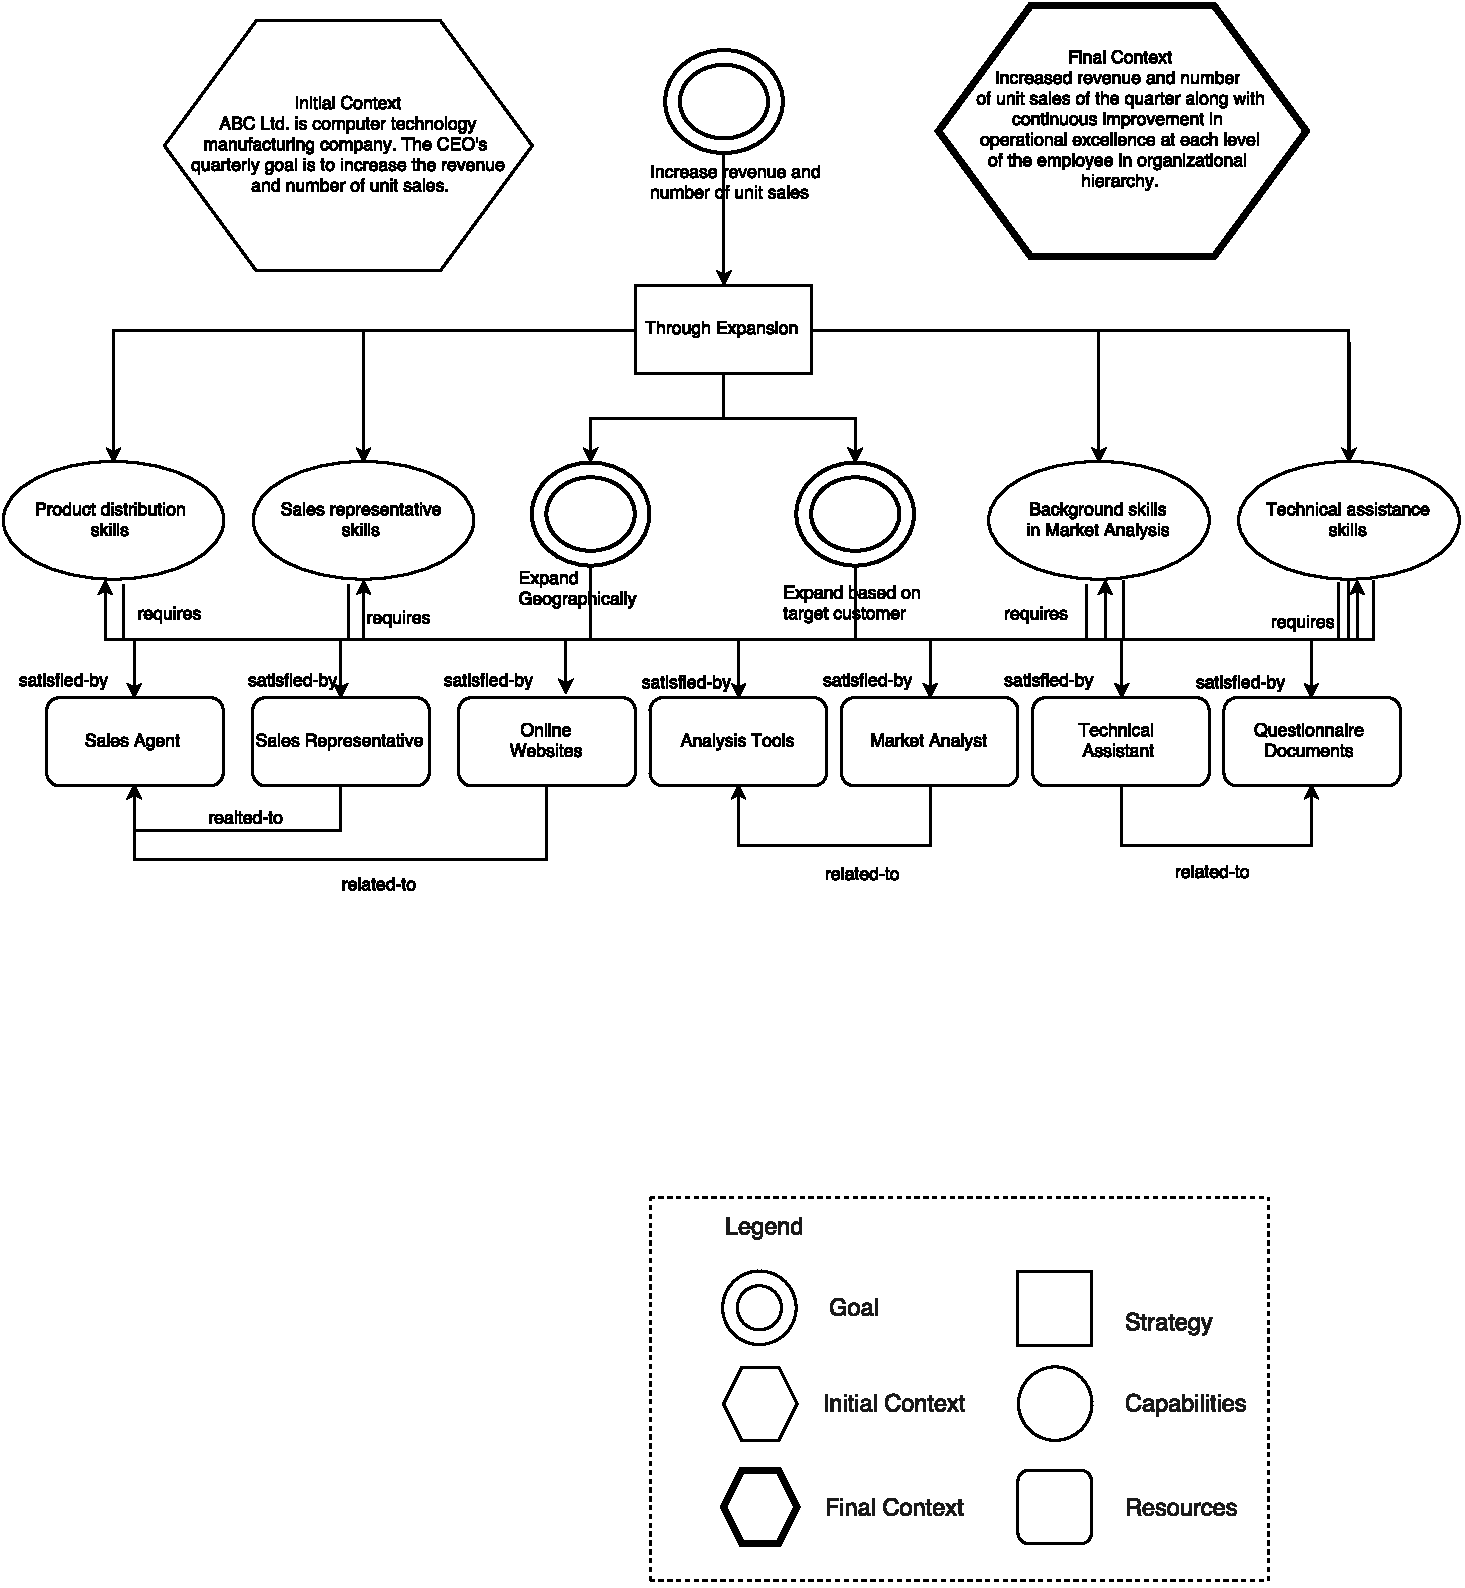
\includegraphics[width=\textwidth]{StrategyView.pdf}
	\caption{Strategy View}
	\label{fig:strategyview}
\end{figure}

\begin{figure}
	\centering
	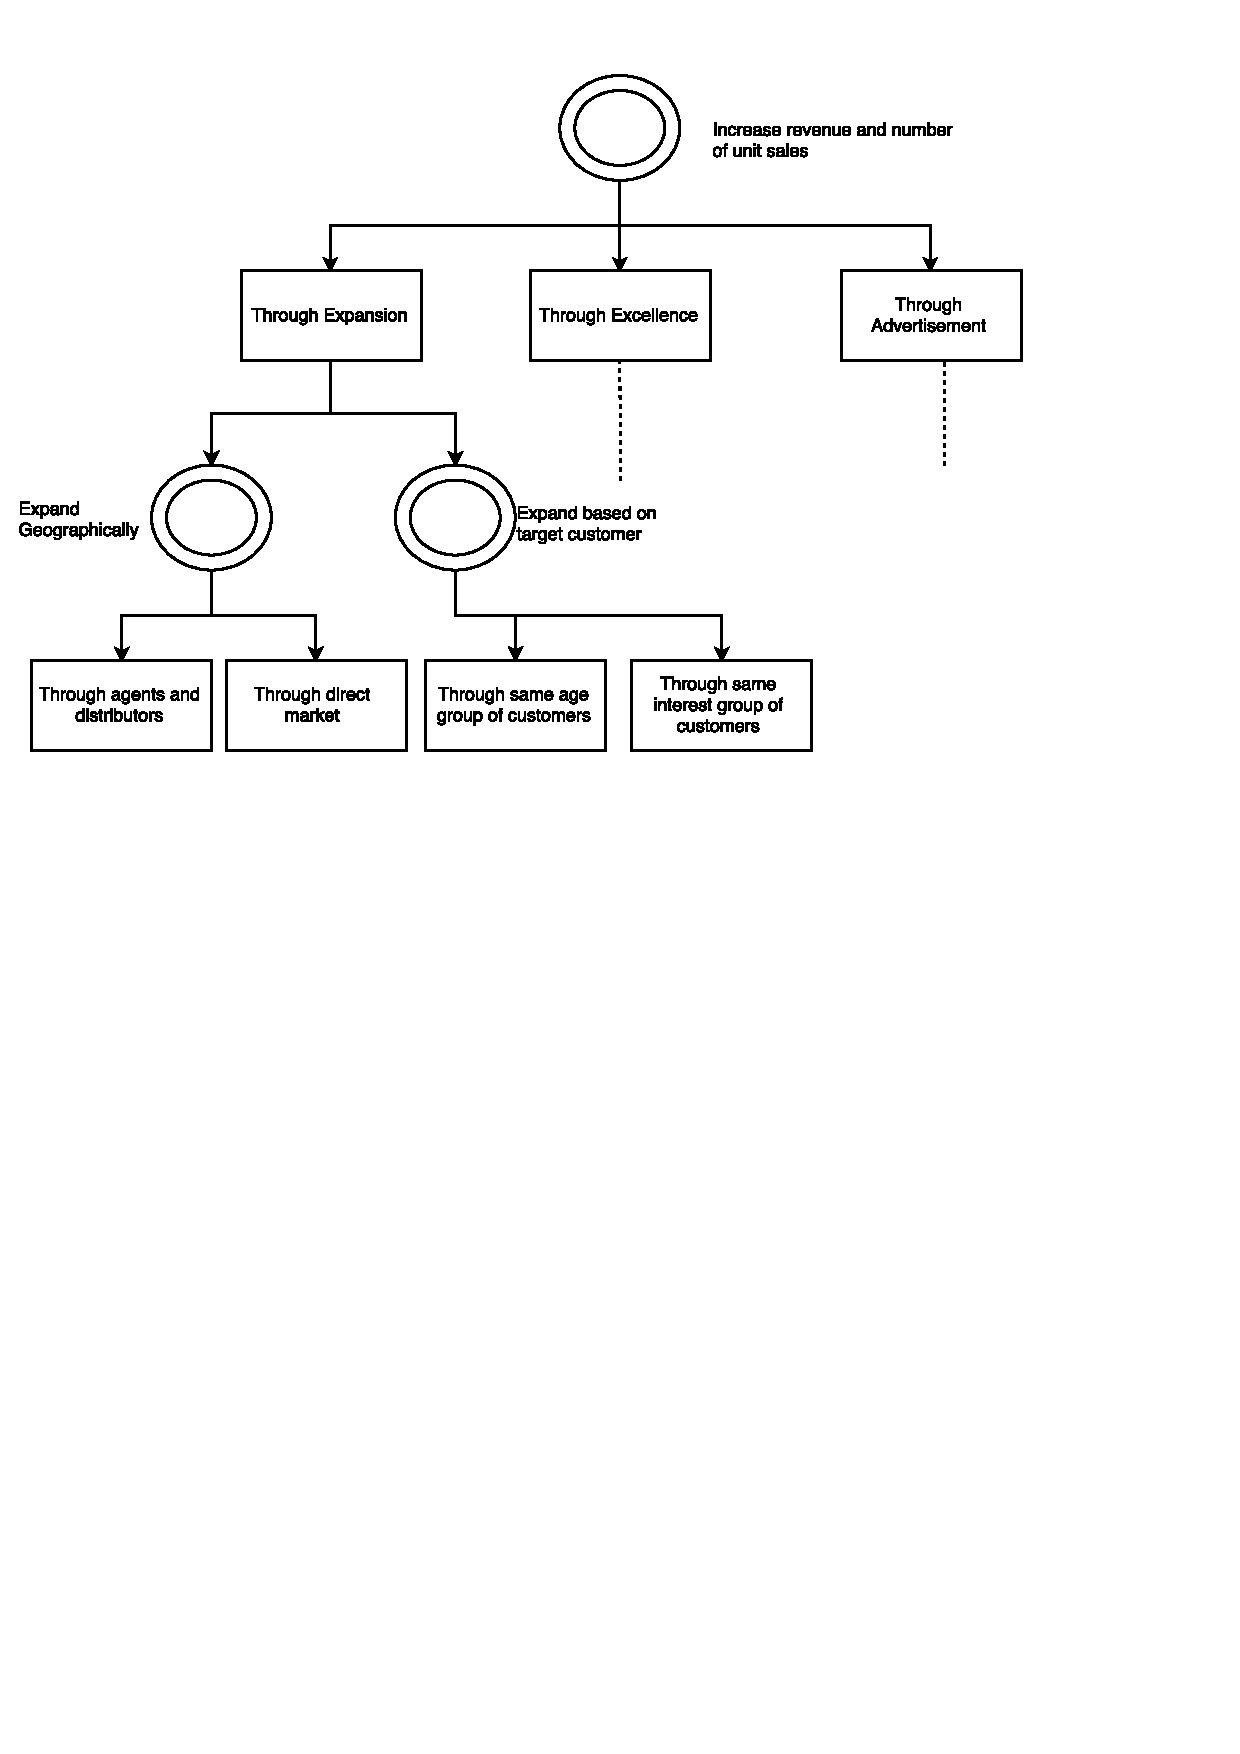
\includegraphics[width=\textwidth]{GoalView.pdf}
	\caption{Goal View}
	\label{fig:goalview}
\end{figure}

%%%%%%%%%%%%%%%%%%%%%%%%%%%%%%%%%%%%%%%%%%%%%%%%%%%%%%%%%%%%%%%%%%%%%%%%%
\section{An Abstract View of Entity Types}
\label{sec:entities}
%%%%%%%%%%%%%%%%%%%%%%%%%%%%%%%%%%%%%%%%%%%%%%%%%%%%%%%%%%%%%%%%%%%%%%%%%
 --- This section discusses in details, about each entity types of the motivating scenario and 
 their images---
 

%%%%%%%%%%%%%%%%%%%%%%%%%%%%%%%%%%%%%%%%%%%%%%%%%%%%%%%%%%%%%%%%%%%%%%%%%
\subsection{Organizational Intentions} 
\label{sec:intentions}
%%%%%%%%%%%%%%%%%%%%%%%%%%%%%%%%%%%%%%%%%%%%%%%%%%%%%%%%%%%%%%%%%%%%%%%%%


%%%%%%%%%%%%%%%%%%%%%%%%%%%%%%%%%%%%%%%%%%%%%%%%%%%%%%%%%%%%%%%%%%%%%%%%%
\subsection{Organizational Strategies} 
\label{sec:strategies}
%%%%%%%%%%%%%%%%%%%%%%%%%%%%%%%%%%%%%%%%%%%%%%%%%%%%%%%%%%%%%%%%%%%%%%%%%

%%%%%%%%%%%%%%%%%%%%%%%%%%%%%%%%%%%%%%%%%%%%%%%%%%%%%%%%%%%%%%%%%%%%%%%%%
\subsection{Organizational Capabilities}
\label{sec:capabilities}
%%%%%%%%%%%%%%%%%%%%%%%%%%%%%%%%%%%%%%%%%%%%%%%%%%%%%%%%%%%%%%%%%%%%%%%%%



%%%%%%%%%%%%%%%%%%%%%%%%%%%%%%%%%%%%%%%%%%%%%%%%%%%%%%%%%%%%%%%%%%%%%%%%%
\subsection{Organizational Resources} 
\label{sec:resources}
%%%%%%%%%%%%%%%%%%%%%%%%%%%%%%%%%%%%%%%%%%%%%%%%%%%%%%%%%%%%%%%%%%%%%%%%%

Each resources has different types of relationship with other resources based on how they communicate with other resources \cite{Sungur2015}. For example in our motivating scenario described in Section \ref{sec:scenario} has one of the sub-intention as \textit{through excellence}. This sub-intention can be achieved by providing skills improvement training to the employees or by recuriting newly skilled employee. Here the manager has permissions to decide whether to improve skills of existing employee or recruit new employee. But the team lead has restricted permission like what type of skills are required for the project based on decision of manager. The Informal Process Essentials (IPE) approach proposed by Sungur et al. \cite{Sungur2015}, paves the way to create models with definitions of key actors e.g manager, team lead and definitions of suppoting resources such as Mediawiki \footnote{http://www.mediawiki.org/}.



%%%%%%%%%%%%%%%%%%%%%%%%%%%%%%%%%%%%%%%%%%%%%%%%%%%%%%%%%%%%%%%%%%%%%%%%%
\subsection{Organizational Processes} 
\label{sec:processes}
%%%%%%%%%%%%%%%%%%%%%%%%%%%%%%%%%%%%%%%%%%%%%%%%%%%%%%%%%%%%%%%%%%%%%%%%%

%%%%%%%%%%%%%%%%%%%%%%%%%%%%%%%%%%%%%%%%%%%%%%%%%%%%%%%%%%%%%%%%%%%%%%%%%
\subsection{Informal Process Instances} 
\label{sec:ipinstances}
%%%%%%%%%%%%%%%%%%%%%%%%%%%%%%%%%%%%%%%%%%%%%%%%%%%%%%%%%%%%%%%%%%%%%%%%%